\documentclass[a4paper,10pt,twocolumn,oneside,openright,final]{memoir}
\usepackage[english]{babel}
\usepackage{etex}
\usepackage{times}
\usepackage{setspace}
\usepackage{inputenc}
\usepackage{amssymb}
\usepackage{amsfonts}
\usepackage[pdftex]{graphicx}
%\usepackage{subfigure}
\usepackage{alltt}
\usepackage{moreverb}
%for more info on hyperref package see http://en.wikibooks.org/wiki/LaTeX/Packages/Hyperref
\usepackage[pdftex,colorlinks=true,linkcolor=blue]{hyperref}
\usepackage{eso-pic}
\usepackage{transparent}
\setlength{\columnsep}{3em}

\usepackage{wrapfig}
\usepackage{subfig}
\usepackage{alltt}
\usepackage{moreverb}
% tikz related packages to provide scalable graphics
\usepackage{tikz}
\usetikzlibrary{calc,mindmap,backgrounds,positioning,arrows,shapes,shapes.arrows,shapes.misc,automata,petri,patterns,scopes,chains,matrix,decorations.pathmorphing,shadows,calc}


\usepackage{geometry}
\geometry{hmargin={15mm,15mm},vmargin={15mm,20mm}}

\usepackage[pages=some]{background}

\backgroundsetup{
  scale=1.2,
  angle=0,
  opacity=0.4,
  contents={
    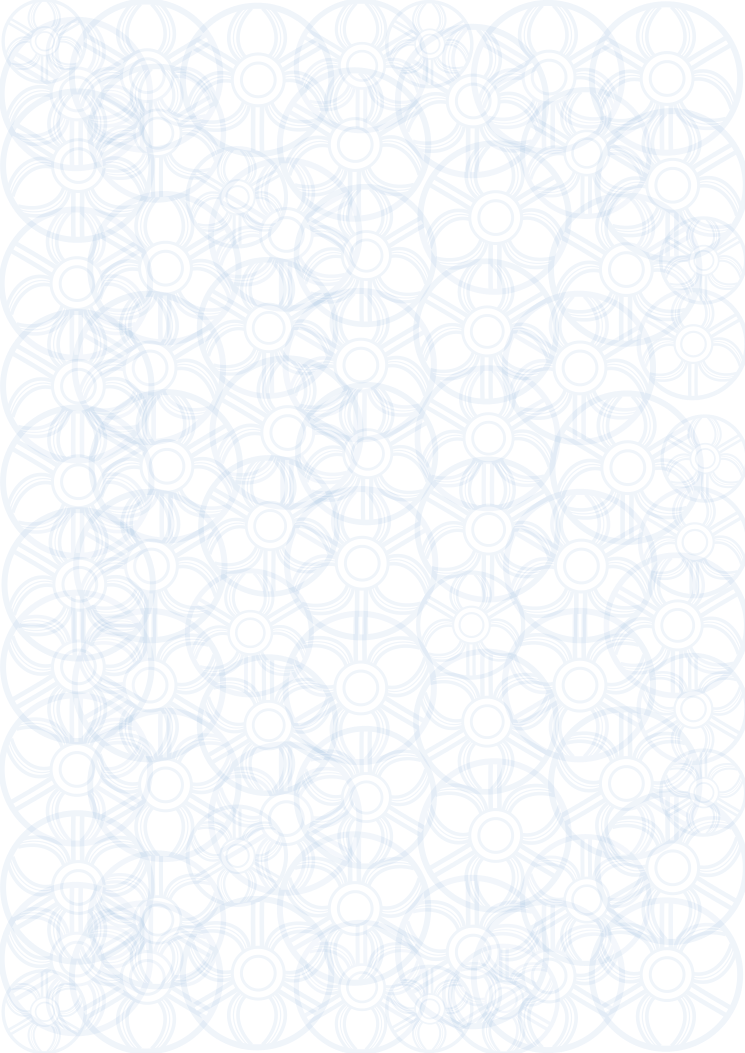
\includegraphics[width=1.1\paperwidth,height=1.1\paperheight, keepaspectratio]{images/00-background.png}}
}


%%%%%%%%%%%%% copyright %%%%%%%%%%%%%%
\title{Trident Genesis Platform}
\author{Fielden Management Services Pty. Ltd.}
\usepackage{hyperref}
\usepackage{hyperxmp}
\hypersetup{
    pdftitle={Trident Genesis Platform},
    pdfauthor={Fielden Management Services Pty. Ltd.},
    pdfsubject={A hight level overview of key principles and advantages.},
    pdfcopyright={Copyright (C) 2019 by Fielden Management Services Pty Ltd.  All rights reserved.}
}

\usepackage{xcolor}
\makeevenhead{headings}%
    {\thepage}{}{\slshape\bookname~\thebook\qquad\partname~\thepart\qquad\leftmark}
    \makeoddfoot{headings}{\slshape\rightmark}{\color{gray}Copyright (C) 2019 by Fielden Management Services Pty Ltd.  All rights reserved.}{\thepage}
	\makeoddhead{headings}{\slshape\rightmark}{}{}


\copypagestyle{headingsnobook}{headings}
\makeevenhead{headingsnobook}{\thepage}{}{\slshape\leftmark}

\begin{document}

%\BgThispage

\subsection*{What is Trident Genesis platform?}
  Trident Genesis (TG) platform is a technology for developing Enterprise Application Software in a domain-driven way.
  TG incorporates over 30 years of experience in delivering enterprise-grade software solutions at a software architecture level to deliver \emph{extensible}, \emph{maintainable}, \emph{interoperable} and \emph{portable} software.
  In essence, TG encapsulates \emph{accidental complexity} of low-level technology in order to enable software engineers to better harness the
  \emph{essential complexity} that stems from a target business domain.

  \vspace{3 mm}
  \noindent Businesses, even from the same industries, are often unique.
  Their unique operational processes and business practices provide a way to serve their customers better and be competitive.
  Modelling business processes as a functional software system provides a way to systematise them to run \emph{efficient}, \emph{effective} and \emph{adaptable} business operations.

\begin{figure}[!h]
    \vspace{-5pt}
    \centering
    \begin{tikzpicture}[node distance=1cm, auto, opacity=0.8, scale=0.7, every node/.style={scale=0.7}]
      \tikzset{
	  mynode/.style={rectangle,rounded corners,draw=black, top color=white, bottom color=blue!50,very thick, inner sep=1em, minimum size=3em, text centered, text=blue!50!black},
	  platform/.style={rectangle,rounded corners,draw=black, top color=white, bottom color=green!50!white,very thick, inner sep=1em, minimum size=3em, text centered, text=green!50!black}
      }
      \node at (1, 1) [mynode] (ap1) {Application};
      \node at (1.7, 1.7) [mynode] (ap1) {Application};
      \node at (2.4, 2.4) [mynode] (ap1) {Application};

      \def\platformpath{-- +(5cm,0cm) -- +(5cm,2cm) -- +(3cm,2cm) -- +(3cm,2.5cm) -- +(4cm,2.5cm) -- +(2.5cm,3.5cm) -- +(1cm,2.5cm) -- +(2cm,2.5cm) -- +(2cm,2cm) -- +(0cm,2cm) -- cycle}
      \draw (-1,-3.3) [platform] \platformpath
	    node [below,text width=7em, text centered,xshift=2.2cm,yshift=0.8cm] {Trident Genesis Platform};
    \end{tikzpicture}
    \vspace{0pt}
  \end{figure}

  \noindent A typical software development workflow with TG encompasses: modelling a business domain (declarative ontological aspect), implementing core business rules (imperative aspect) and configuring user interfaces.
  These steps are facilitated by high level abstractions, APIs and architectural patterns that the platform provides.
  Essentially, TG enables software engineers to concentrate on the modelling of business domains, which improves their productivity and ensures a greater quality and value of TG-based solutions to the business.


 \subsection*{Principles and Advantages}
  	TG is designed to ensure that TG-based software systems are \emph{extensible}, \emph{maintainable}, \emph{interoperable} and \emph{portable}, and facilitate communication between different stakeholders by incorporating the following principles and approaches.

\subsubsection*{Unique object-oriented architectural style for uniform modelling of a business domain}
	One could argue that commanding a programming language is relatively easy.
  	However, object-oriented design is a different story.
  	It takes many years to become an experienced software architect.
  	TG provides a well-defined architectural style that automates low-level technical tasks, and most importantly incorporates a unique architectural approach with its roots in the theory of conceptual modelling of information systems to enable uniform modelling of business domains.
	The platform ensures that all TG-based systems follow exactly the same development and modelling style, which leads to structural and behavioural uniformity of the final solution.
  	This protects software engineers from a multitude of programming errors, and facilitates agile development processes with improved capacity to onboard new software engineers later in a product life cycle.

    \begin{figure}[!h]
    %\vspace{20pt}
    \centering
    \begin{tikzpicture}[>=latex', scale=1.0, every node/.style={scale=1.0}]
      \tikzset{
	  outercore/.style={circle, fill=blue!50!white, inner sep=0em, minimum size=0.6cm},
	  core/.style={circle, shade, ball color=green!50!white, inner sep=0em, minimum size=0.3cm},
	  score/.style={circle, fill=green!50!black, inner sep=0em, minimum size=0.3cm},
	  outer/.style={circle, fill=blue!50!white, inner sep=0em, minimum size=2.3cm},
      }
      \begin{scope}[opacity=0.8]
	\node (o) at (0, -0.25) [outer, opacity=0.3] {};
	\fill[circle, color=green!50!white] (0, -0.25) circle (0.7cm) node [below,text=blue!50!black,yshift=1.1cm] {Synthesised Domain Entity Model};
      \end{scope}

      \begin{scope}[scale=0.3,opacity=0.8]
	\node (t) at (0,0) [outercore, opacity=0.5] {};
	\node at (0,0) [core, opacity=0.5] {};

	\node (r) at (1,-1.2) [outercore, opacity=0.5] {};
	\node at (1,-1.2) [core, opacity=0.5] {};

	\node (l) at (-1,-1.2) [outercore, opacity=0.5] {};
	\node at (-1,-1.2) [score] {};
      \end{scope}

      \node (pe) at (1.3, 1.5) [text=green!50!black,scale=0.8] {Persistent Entities};
      \fill [green!50!black,->,out=-100, in=80] (pe.south) edge (t.north);
      \fill [green!50!black,->,out=-100,in=80] (pe.south) edge (r.north);

      \node (se) at (-1.3, 2) [text=blue!50!black,scale=0.8] {Synthesised Entities};
      \fill [blue!50!black,->,out=-60,in=160] (se.south) edge (l.west);
      \fill [blue!50!black,->,out=-80,in=160] (se.south) edge (o.west);
    \end{tikzpicture}
    \vspace{-60pt}
  \end{figure}

\subsubsection*{Single programming language (Java)}
	Modern software technology stacks are diverse and complex.
	Separate layers often follow different approaches, and may require different programming languages.
	Databases require SQL knowledge, constructing Web UI requires a knowledge of HTML, CSS and JavaScript, the middleware requires some other language such as Java, Scala or C\# as well as associated frameworks.
	All of this makes software engineering a complex multidisciplinary activity.
	Adding the requirement for proper modelling of an actual business domain on top of that only complicates the situation and explains why so many software projects do not get completed or collapse under their own weight during a maintenance life cycle.
	That's why one of the core TG principles is \emph{one language to rule them all}.
	This single language is Java, one of the most popular programming languages.
	Software engineers that know Java can use TG to concentrate on building a core business value to deliver \emph{extensible}, \emph{maintainable}, \emph{interoperable} and \emph{portable} software by relying on TG's capability to execute domain models, and without delving deep into the underlying technology stack.
	TG does not require any special tools like many ``low-code'' technologies.
	Software engineers can continue using their favourite Java IDE and take advantage of interactive debugging, static code analysis tools and source code version control systems.

\subsubsection*{Optimised for relational databases}
	TG platform was developed inside-out -- this is the solution we use to deliver mission critical EAM and ERP systems to our customers.
	It provides optimised integration with relational databases such as Oracle, SQL Server and PostgreSQL, and utilises domain models to dynamically optimise queries and adjust to data usage patterns at runtime.
	Instead of using SQL, which does not fit well into the object-oriented way of thinking, the platform provides Entity Query Language (EQL), which is an embedded domain-specific language for expressing data queries in a natural manner for traversing object graphs.

\subsubsection*{Automated business domain model verification by means of domain-driven testing}
	The notion of automated testing is frequently used to ensure the quality of software systems.
	Unfortunately, often unit and integration testing is an afterthought and software technology stacks need to be extended with additional facilities to enable such testing.
	TG platform provides first-class support for unit and integration testing in a domain-driven way.
	Unit and integration tests represent verification rules and the domain-driven testing in TG ensures their evolution alongside the underlying business domain model.
	This makes Test Driven Development (TDD) a natural fit to developing software with TG.

\subsubsection*{Continuous validation and integration of business domain models during the system lifecycle}
	TG platform stands on the shoulders of giants.
	This is no different when it comes to continuous integration (CI) and validation of TG-based software systems.
	The domain-driven testing is fully compatible with modern CI tools like Jenkins and Hudson.
	Thus, the systems lifecycle can be fully integrated with one of CI the tools to ensure continuous validation of the business domain models underpinning a software system.

\subsubsection*{Direct interaction and manipulation of business domain models}
	The \emph{worldview metaphor} is fundamental to TG-based solutions, where the \emph{world} is an actual business domain model.
	This means that software engineers and the end system users have direct access to the same model!
	While engineers interact with models at the code level and can enhance them, system users can interact with and manipulate exactly the same models through the UI.
	Users can review domain entities and their relationships, and enhance them with calculated properties from the UI for the purpose of data interrogation, analysis and reporting.
	This significantly reduces the misconceptions about the system's actions, structure and logic, and empowers users to truly utilise the capabilities of the underlying domain model.
	Instead of using external tools for accessing raw data in databases, users are provided with an embedded business intelligence capability to interact with the data through a well defined domain model -- entities and their properties.
	\begin{figure}[!h]
  		\centering
  		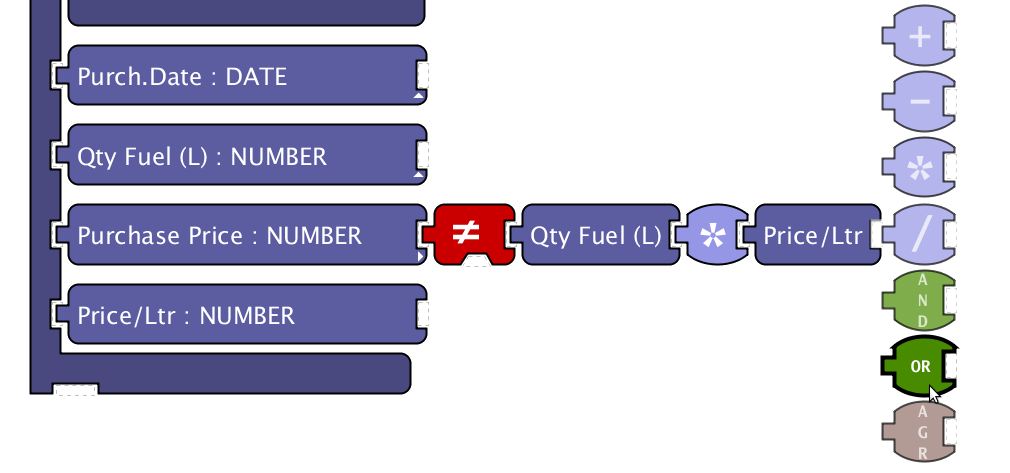
\includegraphics[scale=0.20]{images/01-rulesarea-suggestionmenu.png}
		\vspace{-30pt}
  	\end{figure}

%\BgThispage

\subsubsection*{Responsive HTML5 clients}
	TG provides an embedded domain specific language for defining a responsive Web UI.
	All UI concepts are based on the domain modelling principles to reinforce the worldview metaphor, and follow the Google Material Design spec to deliver a responsive and consistent User Experience (UX) across devices of multiple and varying form factors.
	The TG presentation layer is based on Web Components (built with Google Polymer), which enables reuse and integration of in-house and $3^{rd}$ party components.
	TG offers a \emph{search-first} approach to UX design that provides users with sophisticated first-class data retrieval tools supporting model-driven selection criteria, value autocompletion, ranges, meta-conditions (e.g. missing value, this year, previous fortnight), aggregations and sorting of the result sets.


\subsubsection*{A software engineering tool to facilitate change management}
	Agile, Kanban, Scrum, FDD, TDD\ldots all of these and more are the management techniques, methodologies and methods to ensure the development of high quality software and its timely delivery.
	These project management approaches exist for a good reason and there are multiple tools that assist with their implementation and practicing.
	This, however, is only one side of the coin.
	Implementing a proper process management method does not solve the problem of software engineering.
	It does not take away technical needs and issues that arise during software construction.
	It can only help in mitigating them.
	That is why having an appropriate software construction tool that works well with the process management method is vital to the success of any software project.
	Using TG elevates software engineers to the level of a target business domain, forces them to understand business needs and implications of software systems that are being developed, establishes a ubiquitous business domain language to facilitate communication between project stakeholders, and establishes a well-defined change management process.

\subsubsection*{Robust Security}
	TG provides industrial grade security, which includes HTTPS communication, the use of key-stretching PBKDF2-based password hashing, mutating session authenticator strategy, and reduced sign-on with support for both trusted and untrusted devices.
	There is support for multi-factor authentication scheme, as well as declarative fine-grained authorisation with muti-role support and pluggable backends (e.g. LDAP), user-based data filtering.

\subsubsection*{Cloud-ready}
	Software systems built with TG are cloud-ready and can be deployed as Docker containers.
	The platform employs RESTful architecture to structure application web-resources, and can expose underlying domain models via the GraphQL API.
	This ensures clean separation between different business domain boundaries and UI resources, and provides excellent capacity for scalability.

\subsubsection*{Complete application development lifecycle}
	One of the key meta-features of the Trident Genesis platform is its ability to support a complete lifecycle for developing software systems.
	This was one of our essential goals.
	Otherwise, there would always be some low level technical aspects to software development that interrupt high level business domain-oriented development thinking.
	Thus, the development of software systems with TG covers all that is required for end-to-end software construction.
	This includes orthogonal aspects such as unit and integration testing, build and installation, business model design and database integration, UI definitions, application security, scalability and more.

\end{document}

